%%==================================================
%% chapter01.tex for BIT Master Thesis
%% modified by yang yating
%% version: 0.1
%% last update: Dec 25th, 2016
%%==================================================
\chapter{绪论}
\label{chap:intro}
\section{本论文研究的目的和意义}

近年来,随着社会各方面的快速发展,移动互联和社交网络的普及,全球的数据量以指数级快速增长,人类社会已经迈入大数据时代\upcite{Lynch2008Big,Li2012Research,Wang2013Network}。随着计算机信息技术和多种新兴技术如云计算、物联网、分布式计算的快速发展,对大数据处理和挖掘成为可能,从浩瀚数据中挖掘出有用的知识,成为了学术界和工业界的研究的热点。

大数据是什么,麦肯锡全球研究所给出的定义是\upcite{McKinsey2011}:大数据一种数据集合,这种数据集合规模很大,在获取、存储、管理、分析等方面大大超出了传统数据库软件工具能力的范围,并且具有海量的数据规模、快速的数据流转、多样的数据类型和较低的价值密度四大特征。大数据数据量巨大,已经超出传统数据库的存储能力,目前,个人计算机硬盘容量可达TB量级,一些企业的数据量接近EB量级。大数据的处理速度快,因为数据量庞大,如何在海量数据中快速得到有用信息是十分重要的。大数据的种类繁多,数据可以被分为结构化数据和非结构化数据,结构化数据包括常见的关系数据库存储的数据类型,非结构化数据是数据结构不规则的数据,如网络日志数据、音频数据、视频数据、图片数据等等。非结构化数据的存在对数据的处理能力提出了更高的要求。大数据的数据量大,而价值密度却低。一般而言,价值密度和数据总量的大小成反比。所以,如何从海量的低价值的数据中挖掘出更有价值的信息,是一个重要的研究内容。另外,大数据还具有分布极其不规律,有用的信息隐藏程度很深等特点。从海量数据中,可以提炼出大知识,从而可以对人类社会带来很大的价值,这是大数据带来的机遇与挑战。

相比于传统数据的处理,大数据的计算模式主要分为两种,批量计算和流式计算。批量计算是将数据先存储下来,再对数据进行分批次的计算,这种方式对数据计算的实时性要求不高,主要适用于不需要及时处理数据的场景,但是其处理数据的精度和全面性有保证。现在常用的批处理计算系统主要有Apache的Hadoop框架\upcite{White2009Hadoop}。与之相反,流式计算不会先将数据存储起来,而是直接对数据进行计算,因此对数据的计算速度有很高的要求。流式计算一般直接对数据在内存中进行计算,实时性强,但对数据的处理的精确度要求较低。在流式计算中,只对数据进行一次读取,不存在再次读取情况,这是流式计算的“one-pass”原则。由此可见,批量计算和流式计算相互补充,为了达到更好的处理效果,一般场景下,可以将两种计算模式结合使用,结合两者的优势来处理数据。

现如今,数据呈爆炸式增长,流式数据的应用越来越广泛,流式计算的重要性越来越多地显示出来。数据的流式计算可以广泛地应用于生活和生产的多个方面,如金融市场,天气气象领域,航空航天领域,传感器网络和流量监控领域等等。流式数据是指按照时间顺序不断增加的动态数据序列,具有潜在的无限体积,其计算的实时性要求高,对精度的要求比较宽松\upcite{李圣2016大数据流式计算系统研究综述}。目前,主流的流式计算系统有Twitter的Storm,LinkedIn的Kafka\upcite{kafka2013, Auradkar2012Data},Yahoo的S4(Simple Scalable Streaming System)\upcite{Chauhan2012Performance, Xhafa2015Processing, Neumeyer2011S4},以及传统行业金融领域中比较知名的StreamBase\upcite{Patrizio2006StreamBase}和Borealis\upcite{Abadi2005The}等。

由以上可知,流式数据作为大数据的一种重要的形态,在多个领域中有着非常广泛的应用前景,但该技术作为近几年快速发展应用的技术,仍然具有很大的挑战,主要在数据的收集、存储、处理和可视化上面。流式数据的实时性和庞大的数据量,连续快速到达的特点,以及在线分析的应用需求,带来了挑战,也带来了很多机遇\upcite{孙玉芬2007流数据挖掘综述}。

\section{国内外研究现状及发展趋势}
%\label{sec:***} 可标注label
目前,随着各个领域中处理数据量的增大,流式计算模式的普遍应用,流式数据的处理越来越广泛,国内外很多大学和研究机构都对数据流的管理系统进行了研究,其中一种流式数据分析与处理的典型模型结构如图\ref{fig:fig1}所示\upcite{于戈2006数据流分析}。从中可以看出流式数据的处理系统模型在理论上主要包括两大类,一类是流式数据的预处理,一类是流式数据的数据挖掘。

流式数据分析与挖掘系统模型的数据来源是流式数据的采集器,传感器是一种常见的采集器,比如要获取发动机的数据,则使用发动机上的传感器进行采集。流式数据的预处理包括几部分,拿到原始数据后,可以根据实际处理需要,对原始数据进行汇总、压缩、降维或者动态索引等操作,得到一个概要的数据集或者是近似的数据集。数据的降维主要发生在数据维数较高的场景中,将高维的数据映射到低维的空间,其中,主成分分析(PCA)方法\upcite{croux2018robust}是一种广泛应用的高维数据的降维方法,该方法通过正交变换,将一组可能存在相关性的变量转换为一组线性不相关的变量,减少数据关系之间的重叠性,通过少数几个主成分来表示多个变量之间的内部结构,重新组合成一组新的互相无关的综合指标来代替原来的指标。数据的压缩可以减少数据的存储量,动态索引可以更快地查找数据。这些预处理操作可以降低时间复杂度和空间复杂度,可以去除原始数据中一些不必要的特征,减少数据中的噪音,对后续的数据处理具有很重要的意义。在数据的挖掘处理中,对数据进行统计分析,可以很好地体现数据的特征,如常见的平均值、方差、均值等特征值的统计;对数据进行趋势分析,可以根据历史数据的变化情况,对将要到来的数据进行预测,多用于金融财务和股价方面的预测;对数据进行频繁模式的挖掘,可以找出频繁地出现在数据集中的模式,比如项集、子序列或者子结构;对数据进行模式匹配,可以在浩瀚数据中找到特定的数据;对数据进行聚类分析和分类分析,可以将无分类的无规律的错综复杂的原始数据分为多类,每个类里的数据具有相似性,反映相同的规律性和特性;而对数据进行异常数据检测,可以找出不符合正常行为模式的数据,在网络入侵、金融欺诈和机器监测等方面具有重要应用。

\begin{figure}
	\centering
	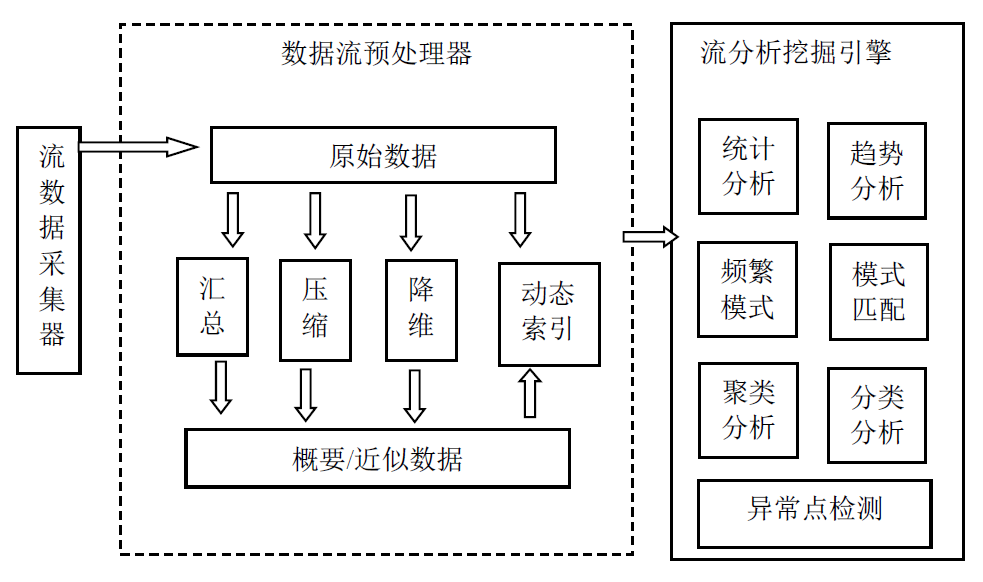
\includegraphics[width=0.75\textwidth]{figures/figure1x1}
	\caption{流式数据分析与挖掘系统模型}\label{fig:fig1}
\end{figure}

流式数据是连续的随着时间产生的数据序列,其中的数据可以是关系元组,也可以是数据项。目前在数据流研究领域存在多种数据流模型,分别有时序模型,现金登记模型和十字转门模型\upcite{孙玉芬2007流数据挖掘综述}。假设流式数据$X$的数据项为 ${x}_{1},{x}_{2},{x}_{3}, ..., {x}_{i}, ...$,数据项序列的下标$i$按顺序递增的,每个下标出现且只出现一次,则

\textbf{时序模型}:\ 每个数据项都代表所描述数据的属性值,$X[i] = {x}_{i}$。

\textbf{现金登记模型}:\ 多个数据项增量地描述数据的属性值,令${x}_{i} = \left(j,{I}_{i} \right)$,其中${I}_{i} > 0$,则有${X}_{i}[j] = {X}_{i-1}[j] + {I}_{i}$。

\textbf{十字转门模型}:\ 多个数据项描述数据的属性值,与现金登记模型的区别是现金登记模型的数据的属性值是一直在增大的,而十字转门模型的属性值可以增大,也可以减小。令${x}_{i} = \left(j,{U}_{i} \right)$,其中${U}_{i}$可以为正数,也可以为负数,则有${X}_{i}[j] = {X}_{i-1}[j] + {U}_{i}$。

其中,时序模型在流式数据的分析和挖掘中应用比较广泛。时序数据的数据项是一个关系元组$\left \langle t,s \right \rangle$,其中,$t$为时间戳,$s$为$t$时刻对应数据的属性值。数据流的数据具有时效性,因此数据携带有时间特征,通常为产生时刻的时间戳。流式数据要求对它进行实时性处理,数据项一旦流过就不复存在,不能再次进行访问,流式数据是源源不断产生的,具有潜在的无限体积,因此不能被全部存储下来。这些都是流式数据的特点。

\section{主要研究内容}
本文主要对流式数据的分析和处理进行研究。针对流式数据的特点,研究异常数据检测和数据压缩的常用算法,探讨在流式计算环境下,如何对算法更好地使用和优化加速,提高流式数据的处理效率。

异常数据检测的任务主要是从数据集中有效地检测出异常数据,异常数据是指在数据集中不符合正常行为模式定义的数据模式,也称为离散点。异常数据在数据集中所占比重小,采样困难,但是其中一般存在重要的信息,或者如果不进行检测,会对后续的处理产生重要的甚至灾难性的影响。比如在工业中,机器发生故障,此时通过异常点检测可以及时发现故障机器,减少生产损失。在日常生活中,电信欺诈和信用卡欺诈等行为已经造成了恶劣的社会影响,通过对正常数据生成模型,通过算法检测异常行为,可以有效地避免欺诈行为的发生,保护财产安全。异常数据检测还可以应用在网站维护方面,如果网站的访问量突然大幅度增加,可能原因是网站被黑客攻击或者被爬虫爬取数据等,所以异常数据的检测,在各个方面都具有实际的应用价值,对其进行研究具有重要的意义。目前为止形成了很多较为成熟且实用的方法,例如基于统计的方法、基于距离的方法和基于聚类的方法等。但是,由于时间复杂度和空间复杂度的影响,部分异常数据检测算法多为静态检测方法,适用于维度较低规模较小的数据集的离线检测,而流式数据大多维度高规模大,并且数据是源源不断到来的,数据量不断动态增长,行为模式可能随时间发生变化,所以在流式计算中,许多成熟的静态异常数据检测算法往往会出现检测结果发生偏差的问题,存在精度不高,运行效率低,不再适用等不足。

由大数据的特点可知,数据的数据量巨大,价值密度很低,对数据进行存储,不但需要耗费比较昂贵的存储资源,而且直接存储价值较低的原始数据没有意义。原始数据常常有噪音干扰,将原始数据直接存储后进行分析和挖掘会消耗大量的计算时间和存储空间,而且也会影响算法的准确性和可靠性。对原始数据进行压缩,可以减少数据的存储空间,节省存储资源,减少存储和后续的计算代价,而且数据压缩不计较细节上的差异,用整体数据的一些特征点来刻画整个数据的主要形态,保留这些主体特征,反应了数据的自身特点。数据压缩可以通过控制压缩度来实现不同的精度层次上的搜索和匹配,更能符合大多数领域只关心数据的变化规律或模式的需求。因此,数据压缩是数据预处理环节中重要的一项内容,具有重要的研究意义。在流式计算中,数据流是源源不断持续增长的,在对数据进行压缩时,数据产生的速度很快,如果压缩花费的时间较多,数据的处理不及时,未处理的数据容易拥塞聚集,最后很可能造成数据丢失的严重后果,因此在流式计算中,对压缩算法进行加速有很重要的意义。

本文主要研究流式数据的数据压缩和异常数据检测的时效性问题,来满足流式数据数据规模大,实时性强的特征,以及在线处理的要求。具体来说,针对流式数据的压缩与异常数据检测,完成以下工作:

第一,针对增量LOF算法在流式数据处理中存在的问题,提出了一种改进的增量LOF快速异常数据检测方法,该方法将数据的分布空间进行划分,将数据点映射到对应的网格单元中,可以有效解决流式数据数据量巨大无法在内存中存储计算的问题,而且减少了计算量。在此基础上,将同一网格内的数据点集中到中心一点,对数据点进行基于密度的异常数据检测,这种方法一方面可以减少数据的存储量,另一方面减少了需要进行距离运算的对象,大大减少了计算量,具有很好的时效性和较少的空间消耗。

第二,根据流式数据在线压缩的要求,采用滑动窗口算法与分段多项式拟合算法来对数据进行压缩。针对时序数据的采样时间是否是周期的,分析在多项式拟合中计算多项式系数时所用的最小二乘法的过程,分别采用缓存方法和增量计算的方法,减少计算量,来对数据压缩进行加速。

第三,通过实验,验证了本文针对数据压缩和异常数据检测提出的加速算法的有效性,减少了计算时间,保证了流式数据处理的高实时性。针对基于LOF方法的快速异常检测算法,通过实验对比,验证了本文的算法可以很好地适用于流式计算环境中,并且取得较好的结果,并且处理数据的速度更快,运行内存更小。针对数据压缩的加速   算法,通过实验,验证了本文提出的算法在不同多项式次数和不同误差率的情况下,可以很好地减少运行时间。

\section{章节安排}
本文主要分析异常数据检测和数据压缩在流式环境下的主流算法,探求算法的可行性和效率,基于这些算法提出改进,使计算提高效率,减少计算时间,达到加速效果。然后进行实验分析,保证其在实际中可以应用的可行性。本文的章节安排如下。

第一章,绪论,介绍了研究背景和意义,介绍了大数据的定义与特点,并介绍了大数据的计算模式,分为批量计算和流式计算,介绍了流式数据的特点和流式数据的处理计算模型。

第二章,针对异常数据检测方法和数据压缩方法,分别阐述了其应用背景,方法概述,和相关实现方法。这部分主要介绍异常数据检测方法和数据压缩方法的研究现状和主要使用算法。总结了异常数据检测的相关研究成果,介绍了主流的异常数据检测算法,包括基于统计的、基于聚类的、基于距离的和基于密度的方法。并且介绍了经典的算法,如iForest算法,LOF算法等等。总结了经典的数据压缩的方法,包括奇异值分解法、分段线性法、符号表示法和频域法,分析了各种方法优缺点及应用范围。以及很多方法都是应用在静态数据集中的,在流式数据的计算中,该如何改进使用这些方法。

第三章,介绍了异常数据检测方法的LOF方法和适用于流式数据的增量LOF算法,并且基于这两种方法,提出了一种新方法,该方法相比于增量的LOF方法,减少了存储量和计算量,更适合流式数据。

第四章,介绍了分段多项式压缩的方法,首先分析了在静态数据集上如何进行加速计算,然后针对流式数据给出了滑动窗口算法与分段多项式相结合的压缩算法,最后通过分析其压缩过程,对于不同的数据类型,给出了不同的加速计算方法。

第五章,实验章节,主要分为异常数据检测的对比实验和压缩算法的对比实验。异常数据检测算法主要与增量的LOF算法进行对比,压缩算法与原计算方法进行不同多项式次数的时间对比与不同分段方法的时间对比。

最后对论文的主要研究内容进行了总结。